\documentclass[12pt]{article}
 
\usepackage[margin=1in]{geometry}
\usepackage{amsmath,amsthm,amssymb}
\usepackage{fancyhdr}
\usepackage{hyperref}
\pagestyle{fancy}
\usepackage{graphicx}
\newcommand{\N}{\mathbb{N}}
\newcommand{\R}{\mathbb{R}}
\newcommand{\Z}{\mathbb{Z}}
\newcommand{\Q}{\mathbb{Q}}
 
\newenvironment{theorem}[2][Theorem]{\begin{trivlist}
\item[\hskip \labelsep {\bfseries #1}\hskip \labelsep {\bfseries #2.}]}{\end{trivlist}}
\newenvironment{lemma}[2][Lemma]{\begin{trivlist}
\item[\hskip \labelsep {\bfseries #1}\hskip \labelsep {\bfseries #2.}]}{\end{trivlist}}
\newenvironment{exercise}[2][Exercise]{\begin{trivlist}
\item[\hskip \labelsep {\bfseries #1}\hskip \labelsep {\bfseries #2.}]}{\end{trivlist}}
\newenvironment{problem}[2][Problem]{\begin{trivlist}
\item[\hskip \labelsep {\bfseries #1}\hskip \labelsep {\bfseries #2.}]}{\end{trivlist}}
\newenvironment{question}[2][Question]{\begin{trivlist}
\item[\hskip \labelsep {\bfseries #1}\hskip \labelsep {\bfseries #2.}]}{\end{trivlist}}
\newenvironment{corollary}[2][Corollary]{\begin{trivlist}
\item[\hskip \labelsep {\bfseries #1}\hskip \labelsep {\bfseries #2.}]}{\end{trivlist}}
 
\begin{document}
 
\title{Lab 4: Tunneling, Symmetric Client/Servers, and Monitoring}
\author{Duc Viet Le\\
 CS536}
 
\maketitle
 
\begin{problem}{1} \ \\
Testing our code:
	\begin{itemize}
		\item Actual server runs at: \texttt{sslab01} 
		\item \texttt{Tunneld} runs at: \texttt{borg01} 
		\item \texttt{Mytunel} and \texttt{client} runs at: \texttt{Hicks Library}
	\end{itemize}
\texttt{myping/mypingd}: \\
I sent 8 queries uing tunneling and not using tunneling. Below is the performance:
	\begin{center}
		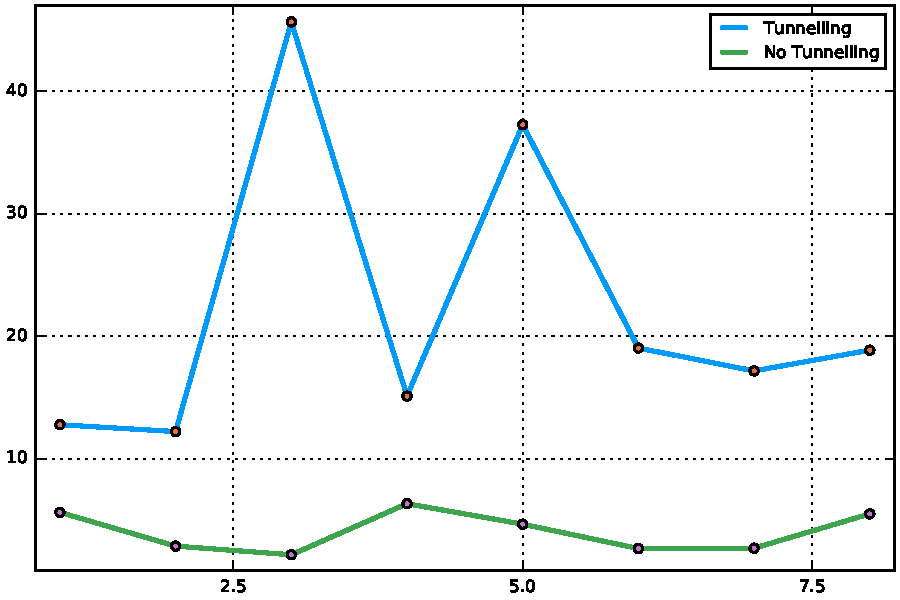
\includegraphics[scale=.5]{1.pdf}	
		\begin{tabular}{c|c|c}
		    & tunnel &  no tunnel \\ \hline
		1   & 12.786 ms&  5.631 ms\\
		2   & 12.225 ms&  2.875 ms\\
		3   & 45.676 ms&  2.167 ms\\
		4   & 15.123 ms&  6.334 ms\\
		5   & 37.285 ms&  4.665 ms\\
		6   & 19.046 ms&  2.674 ms\\
		7   & 17.179 ms&  2.705 ms\\
		8   & 18.874 ms&  5.505 ms\\
		\end{tabular}  
	\end{center}
	\textbf{Discussion:} using tunnel increase the ping number which is understandable because instead of directly transmit our UDP packets, we now need to transmit it through another intermediate server (i.e \texttt{tunneld}) which will increase time. \\

\noindent\texttt{traffic\_rcv/traffic\_snd:} \\
I sent 5 queries uing tunneling and not using tunneling. Below is the performance:
\begin{center}
	\begin{tabular}{c|c|c|c|c|c|c|}
	    & \multicolumn{3}{c|}{tunnel} & \multicolumn{3}{c}{no tunnel} \\ \hline
	    & Time & BPS&  PPS & Time & BPS&  PPS \\ \hline
	1   & 0.109  s& 7766275.5&  920  & 0.116 s& 7270135.5&  861 \\ 
	2   & 0.108  s& 7750229.5&  922& 0.108 s& 7767991.5&  920 \\ 
	3   & 0.108  s& 7784829  &  922& 0.109 s& 7675029.5&  909 \\ 
	4   & 0.108  s& 7781886  &  927& 0.107 s& 7855029.5&  929 \\ 
	5   & 0.109  s& 7731062  &  916& 0.119 s& 7061520.5&  836 \\ 
	\end{tabular}  	
\end{center}
\textbf{Discussion:} There are not many difference between using tunneling and not using tunneling because the throughtputs from \texttt{hicks libary} to \texttt{borg} and \texttt{sslab01} are similar. There will be no bottleneck node. Also, with tunneling, the result seems to be more stable at receiver, and I think the reason is that connection between \texttt{borg} machines and \texttt{sslab01} is more stable compared to connection between \texttt{hick} machine and \texttt{sslab} machines 
\end{problem}


\begin{problem}{2}
	
\end{problem}


\end{document}
